\part{Représenter et homogénéiser dans un format pivot XML TEI les métadonnées Lectaurep}

La première partie du stage comportait une réflexion sur la gestion et la création des métadonnées dans le cadre du projet Lectaurep. Parmi les questions posées : quelles métadonnées sont susceptibles d'être intégrées à la plate-forme eScriptorium lors de l'import des images ? Quelles métadonnées extraire une fois les traitements dans cette même plate-forme effectués ? Par ailleurs, quelles solutions pour modéliser et rendre intéropérables les  métadonnées repérées ? Enfin, sur quelle(s) référentiel(s) s'appuyer ?\footnote{La première mission de stage a été présentée sous la forme d'une \textit{issue} GitLab accessible via le lien : \url{https://gitlab.inria.fr/almanach/lectaurep/documentation/-/issues/1}}. Pour répondre à ces questions plusieurs étapes ont été nécessaires. Dans un premier temps, une présentation de l'ensemble des métadonnées, de leurs référentiels associés et de leur circulation en terme de flux entrants et sortants dans la plate-forme eScriptorium s'est avéré cruciale. En concertation avec l'ensemble des acteurs du projet, nous avons pu repérer un certain nombre de métadonnées à associer aux images lors de l'import et de l'export dans eScriptorium. Dans un second temps, nous avons posé les avantages de les agréger dans un format pivot XML avec une spécification TEI (\textit{Text Encoding Initiative}), devant permettre à terme d'échanger des ressources entre différents systèmes d'informations de Lectaurep. Il a fallut mettre en avant les atouts du référentiel TEI, dans un contexte archiviste, en vue de la continuation du projet Lectaurep sur le long terme. Nous aborderons ce point dans le chapitre 3. Une fois les définitions et les questionnements posés, nous avons pu préparer un environnement propice au développement \inquote{agile} de ce format pivot, afin de garantir sa future évolution et expérimenter une première formalisation dans un fichier XML TEI (créé \textit{ex nihilo} pour l'occasion) avec un petit choix de métadonnées. Nous résumerons ces différentes phases logiques dans le chapitre 4.


\chapter{Enjeux et problématiques liés aux métadonnées et à la TEI dans le projet Lectaurep}

\section{De l'importance de l'interopérabilité des formats de données}

\subsection{Données, métadonnées, interopérabilité et format pivot : définitions et objectifs pour Lectaurep}

\subsubsection{Rappels généraux sur les données et les formats}

On défini généralement la \textbf{donnée} comme \inquote{un terme utilisé, en informatique, pour désigner une information}\footnote{Définition issue de \cite{noauthor_abrege_2020}.}, soit le matériau de plus bas niveau manipulé par un utilisateur sur un ordinateur. On parle alors de \textbf{métadonnées} pour traiter d'une information structurée de nature technique et/ou de gestion et/ou de description servant à décrire les caractéristiques d'une donnée brute en vue de faciliter son repérage, sa compréhension, sa gestion, son usage ou sa préservation selon les cas. Cependant la frontière entre les deux est perméable : ainsi le nom d'une ville peut être considéré comme une donnée ou une métadonnée selon son contexte d'utilisation. Un chercheur en toponymie considérera ce nom comme une donnée exploitable pour son étude, tandis qu'un archiviste effectuant un inventaire le verra comme le lieu de production du document, soit une métadonnée de provenance. 
Les données sont généralement représentées dans plusieurs types de formats au sein d'un \textbf{système d'information}\footnote{Un système d'information (SI) est un ensemble organisé de ressources (matérielles et logicielles) qui permettent de collecter, stocker, traiter et distribuer les données/métadonnées.} (SI). On caractérise un \textbf{format} comme la manière dont est représenté (codé) un type de données dans un ordinateur. Ainsi du texte brut (\textit{plain text}, reconnaissable par son extension de fichier .txt sera, par exemple, représenté selon le standard d'encodage de caractères Unicode (UTF-8). Cependant, des formats plus sophistiqués existent, à l'instar des langages à balises reconnaissables grâce à leurs chevrons ouvrants et fermants (\citecode{< >}). Les plus connus sont ceux qui descendent du langage SGML\footnote{Le \textbf{SGML} ou \textit{Standard Generalized Markup Language} est un langage de description à balises. Apparu dans les années 1980, il rendu possible l'exploitation des premières DTD (\textit{Document Type Definition}) ancêtre des schémas de déclaration d'éléments et de relations actuels de type RelaxNG. Il est aujourd'hui abandonné au profit de ses descendants HTML, XHTML et XML apparus au moment de l'invention du Web dans les années 1990.} (\textit{Standard Generalized Markup Language}) et maintenu par le W3C\footnote{\url{https://www.w3.org}} (\textit{World Wide Web Consortium}) : pour rendre compte d'une mise en page ou d'une typographie particulière ou de plusieurs données (texte stylisé ou \textit{fancy text}) comme le HTML\footnote{Le \textbf{HTML} ou \textit{Hyper Text Markup language} est le langage de la page web par excellence. Il sert à structurer sémantiquement du contenu et à rendre compte de son apparence. Cependant la mise en page du HTML est souvent réalisée avec le langage de programmation JavaScript (apparence dynamique) et du CSS (\textit{Cascading Style Sheets} pour l'apparence statique et dynamique de la page web).} (\textit{Hyper Text Markup language}). On peut également rendre compte de certains aspects du texte brut via le balisage sémantique en XML\footnote{Le \textbf{XML} ou \textit{Extensible Markup Language} est un langage de balisage extensible, héritier du SGML. Au même titre que son frère HTML, il est reconnaissable par l'usage de chevrons ouvrants et fermants : \citecode{< >}. Sa syntaxe est dite \inquote{extensible} car on peut définir ses propres noms de balises (grammaire). Les objectifs du XML sont l'encodage de ressources textuelles via son système de balises, l'échange de contenus complexes pouvant être représentés sous la forme d'arbres entre systèmes d'informations hétérogènes (intéropérabilité). Un document XML pour être \inquote{valide} doit respecter un schéma défini ou non par l'utilisateur (par exemple, une DTD ou un schéma RelaxNG) et posséder une syntaxe \inquote{conforme}. Ce qui est en fait un langage strict en dépit de son apparence d'\inquote{extensibilité}.} (\textit{Extensible Markup Language}). Un document XML respecte généralement une structure logique. Parmi les règles qui définissent un document XML \inquote{bien formé} ou \textit{well-formed} : les principes d'arborescences par imbrication d'éléments (l'élément enfant héritent des propriétés et attributs d'un élément parent) et non de recouvrement ; chaque balise doit correspondre une balise de fin correspondante ; il existe un seul élément racine (\textit{root element}) ; un élément ne peut posséder deux attributs du même nom. Les principes du langage XML sont résumés dans l'exemple ci-dessous : 
\lstset{language=XML}
\begin{lstlisting}
<?xml version="1.0" encoding="utf-8"?> <!-- déclaration XML obligatoire -->
<elementParent couleur='rouge' position='milieuDroitePage'>
    <unElementEnfant id='1'>du texte</unElementEnfant>
    <unElementEnfant id='2'>encore du texte</unElementEnfant>
</elementParent>
\end{lstlisting}
Le format XML présente des avantages conséquents dans la représentation des données, il permet entre autre :
\begin{itemize}
    \item une bonne lisibilité par l'humain et la machine;
    \item une facilité d'intégration dans des plate-formes et logiciels;
    \item une migration vers d'autres formats;
    \item l'échange de données.
\end{itemize}

\subsubsection{La question de l'interopérabilité en jeu dans Lectaurep}

Derrière ces définitions très généralistes, reposent des enjeux essentiels et concrets pour le projet Lectaurep et les utilisateurs de la plate-forme eScriptorium. Les répertoires de notaires numérisés qui sont importés dans la plate-forme ne sont actuellement accompagné d'aucune, voire de très peu de métadonnées. Dès lors un archiviste qui travaille sur la transcription ou la segmentation d'une image ne sera pas en capacité d'avoir des informations précises issues instruments de recherche (producteur d'un document d'archives, cotes, informations techniques sur l'image). De même un chercheur souhaitera référencer son travail avec un minimum de métadonnées accompagnant sa transcription ou effectuer une requête précise directement dans le texte transcrit automatiquement, en vue d'une analyse concernant les noms d'actes, la fiscalité, les types de graphies etc. %himanis
Lectaurep en tant que projet d'analyse et de reconnaissance de documents (ARD) est confronté au problème de la représentation des données pour couvrir des besoins utilisateurs diversifiés, comme le souligne des chercheurs du LORIA (laboratoire lorrain de recherche en informatique et ses applications) et du laboratoire CNRS/ATILF de Nancy (Analyse et traitement informatique de la langue française) : 
\begin{quote}
    Il existe pour ainsi dire autant de formats de représentation des données que de système de stockage ou de reconnaissance de document. Cette grande diversité est un frein certain à l'échange des données d'un environnement à un autre, d'une plate-forme à une autre et rend souvent les sorties de certains systèmes utilisables uniquement par eux-mêmes.\footnote{\cite{belaid_representation_2007}, pp.1-2}
\end{quote}

\textbf{Normes et spécifications d'encodage -}
Le premier objectif pour Lectaurep est donc celui de l'\textbf{interopérabilité}\footnote{On parle généralement du principe ou de l'objectif FAIR (Facile à trouver, Accessible, Interopérable, Réutilisable) dans une plate-forme pour évoquer le fait que les données doivent être échangeables et identifiables pour permettre des bonnes performances.} des données et des métadonnées dans eScriptorium. Soit la capacité de faire communiquer les données et métadonnées entre-elles. Les données et métadonnées susceptibles d'être importées dans eScriptorium suivent pour l'heure des \textbf{spécifications} très différentes et des formats parfois hétérogènes (même si dans l'ensemble les spécifications répondent à une représentation en XML) car provenant de systèmes d'informations divers. Les spécifications ou standards de représentation des données et de métadonnées répondent généralement à des normes techniques d'échange\footnote{Une \textbf{norme technique} est un référentiel publié par un organisme de normalisation officiellement agréé par l'État via une organisation nationale (comme AFNOR en France) ou internationale (comme ISO - Organisation internationale de normalisation). Le but poursuivi est destiné à harmoniser les pratiques d'un secteur d'activité suivant un cadre commun et à garantir un niveau d'ordre optimal.} de données et de métadonnées selon le contexte d'utilisation. Dans le milieu documentaire, par exemple les normes ISAD(G)\footnote{\textbf{ISAD(G)} (\textit{International Standard Archival Description-General}) ou Norme générale et internationale de description archivistique créé en 1994 sous l'impulsion du Conseil International des Archives (ICA) énonce les grands objectifs et principes de la descriptions archivistique et fourni une liste d'éléments de description que l'on peut employer dans un instrument de recherche, avec la définition de ces éléments et des exemples d'utilisation.} et ISAAR(CPF)\footnote{\textbf{ISAAR(CPF)} (\textit{International Standard Archival Authority Record for Corporate Bodies, Persons and Families}) ou Norme internationale sur les notices d'autorité archivistiques relatives aux collectivités, aux personnes et aux familles, est créé en 1995 par le Conseil International des Archives (ICA). La norme énonce les lignes directrices pour la description d'entités (collectivités, personnes, familles) associés à la production et à la gestion d'archives.} sont généralement utilisés dans le domaine archivistique pour décrire respectivement des fonds d'archives et des producteurs. Dans le monde des bibliothèques, le catalogage repose également sur un ensemble de normes comme l'ISBD\footnote{\textbf{ISBD} (\textit{International Standard Bibliographic Description} ou Description bibliographique internationale normalisée est une norme publié en 1971 et définie par l'IFLA (Fédération internationale des associations de bibliothécaires et d'institutions) pour la description du catalogage).} ou le \textit{Dublin Core} (norme ISO 15836) pour décrire des ressources bibliographiques. 
Omniprésent dans l'informatique documentaire, le langage XML permet alors de structurer informatiquement des informations suivant ces normes. Pour prendre des exemples, ISAD(G) se trouve décliné en standard XML EAD\footnote{\textbf{EAD} (\textit{Encoded Archival Description}) ou description archivistique encodée créé en 1993 et maintenu par la Bibliothèque du Congrès. S'appuyant sur la norme ISAD(G), l'EAD est utilisé pour décrire des fonds d'archives, des collections de manuscrits ou des collections hiérarchisés d'objets (photographies, numérisations, microfilms etc.), mais surtout pour encoder des instruments de recherche. L'ensemble des éléments XML sont présentés sur le site officiel : \url{https://www.loc.gov/ead/} et en français via \url{https://www.ead-bibliotheque.fr}} et ISAAR(CPF) en standard XML EAC-CPF\footnote{\textbf{EAC-CPF} (\textit{Encoded Archival Context - Corporate Bodies, Persons and Families}) s'appuie sur la norme définie par ISAAR(CPF) pour la rédaction des fiches de producteurs (personnes morales ou physiques) d'archives. C'est un schéma maintenu par la Bibliothèque d'État de Berlin et la SAA (\textit{Society of American Archivists}). Les éléments de l'EAC sont diponibles : \url{https://eac.staatsbibliothek-berlin.de}}. Ces standards d'encodage sont généralement disponibles sous la forme d'un schéma de validation XML de type Relax NG\footnote{\textbf{Relax NG} (\textit{Regular Language for XML Next Generation}) est un langage de description de document XML permettant de définir les différentes contraintes qui déterminent l'imbrication des éléments ou la place des attributs dans le document pour passer l'étape de validation. C'est une puissante alternative au langage XML Schema.} ou DTD\footnote{\textbf{DTD} (\textit{document type definition}) ou définition de type de document, est un document XML pour définir un modèle pour des fichiers XML qui réglemente l’imbrication des balises, les noms d’éléments autorisés, la façon dont les attributs sont rattachés aux éléments. C'est un schéma XML moins sophistiqué que le Relax NG et XML Schema.} directement épinglé au document XML pour vérifier la strict validé de ce dernier. 
Si ces standards facilitent l'échange de certains type de données, ces dernières peuvent-elles communiquer entre elles ? Nous verrons dans la partie \ref{Circonscrire un monde de données} en détail les formats et spécifications propres aux données et métadonnées qui nous ont particulièrement intéressés dans le projet. 

\textbf{formats d'import et d'export dans eScriptorium -}
La plate-forme eScriptorium ne gère actuellement que des imports d'images au format .jpg ou .jpeg via une fonctionnalité de type \inquote{Glisser/Déposer} (\textit{Drag \& Drop}) ou via l'URI\footnote{\textbf{URI} (\textit{Uniform Resource Identifier}) ou identifiant uniforme de ressource est une chaîne de caractère identifiant une ressource dans un réseau répondant à une norme du W3C pour le web (Cf. RFC 3986). une URL \textit{Uniform Resource Locator} comme par exemple \citecode{http://www.lectaurep.fr/} est un type d'URI qui identifie la ressource (la page de lectaurep), qui implique la représentation de la ressource en HTML obtenue via le protocole HTTP (\textit{Hypertext Transfer Protocol}, principal protocole de communication client-serveur dans le web).} du manifeste IIIF\footnote{\textbf{IIIF} (\textit{International Image Interoperability Framework}) est une communauté et un ensemble de spécification techniques pour fournir un cadre d'intéropérabilité pour la diffusion et l'échange des images en haute résolution sur le Web. L'API Image permet de définir un service web pour renvoyer une image via une requête HTTP construite à partir d'une URI. Cette URI peut spécifier la région, la taille, la rotation, les caractéristiques de qualité et le format de l'image. Elles sont construites selon les besoins des applications clientes. L'API Présentation est un service web qui renvoie des documents structurés en JSON-LD (\textit{JavaScript Object Notation - Linked Data} qui donnent des informations sur la structure et la présentation de l'objet numérisé ou de la collection d'images. En somme, ce sont toutes les métadonnées accompagnant l'image qui peuvent provenir d'autres fichiers de données. Pour plus de précisions : \url{https://iiif.io})} et les transcriptions dans les formats XML ALTO\footnote{\textbf{ALTO} (\textit{Analysed Layout and Text Object}) est un standard XML rendant compte de la mise en page physique et de la structure logique d'un texte transcrit par reconnaissance optique de caractère (OCR/HTR). On y retrouve les coordonnées de segmentation (\textit{baseline}, polygones etc.), des éléments de forme (type de police etc.), ou encore des métriques (taux de confiance de reconnaissance). Le schéma de ce standard est maintenu par la Bibliothèque du Congrès et la BnF. \url{https://www.loc.gov/standards/alto/}}, XML PAGE\footnote{\textbf{PAGE XML} est le principal format de données utilisé par le logiciel Transkribus, il agrège l'ensemble des données relatives à l'image transcrite, le texte transcrit, les coordonnées de zones de texte, les corrections effectuées etc. Pour comprendre les différences entre le XML ALTO et le XML PAGE on pourra se rapporter \cite{bonhomme_defis_2018}, pp. 46-47. Le schéma est disponible : \url{https://www.primaresearch.org/schema/PAGE/gts/pagecontent/2016-07-15/pagecontent.xsd}} pour reprendre le travail de transcription en cours. En export, on peut récupérer le résultat de sa transcription (pour la sauvegarde notamment) au format XML ALTO, XML PAGE ou au format texte brut. Dès lors, on retrouve un format de fichier par type de données, ce qui présente le désavantage pour l'utilisateur de ne pas avoir accès à un ensemble de données et de métadonnées lors de l'import/export de son travail dans la plate-forme. L'utilisateur devrait pouvoir récupérer à la fois l'image de la numérisation du répertoire de notaires (un URI IIIF ou un chemin vers une ressource stocké localement), le résultat de sa transcription (vérité terrain ou résultat HTR), des métadonnées sur l'archive (producteurs, date, étude de notaire etc.) provenant des instruments de recherche du DMC, l'historique de ses traitements (binarisation, segmentation, transcription etc.) en une fois lors de l'import et de l'export dans eScriptorium.    

\subsubsection{Une solution, le format pivot XML}

La figure \ref{fig:modèle_métadonnées_vise_V4} représente le modèle hypothétique envisagé par Lectaurep pour l'utilisation du format pivot et de ses usages à terme. 
\begin{figure}[h]
    \centering
    \centerline{\fbox{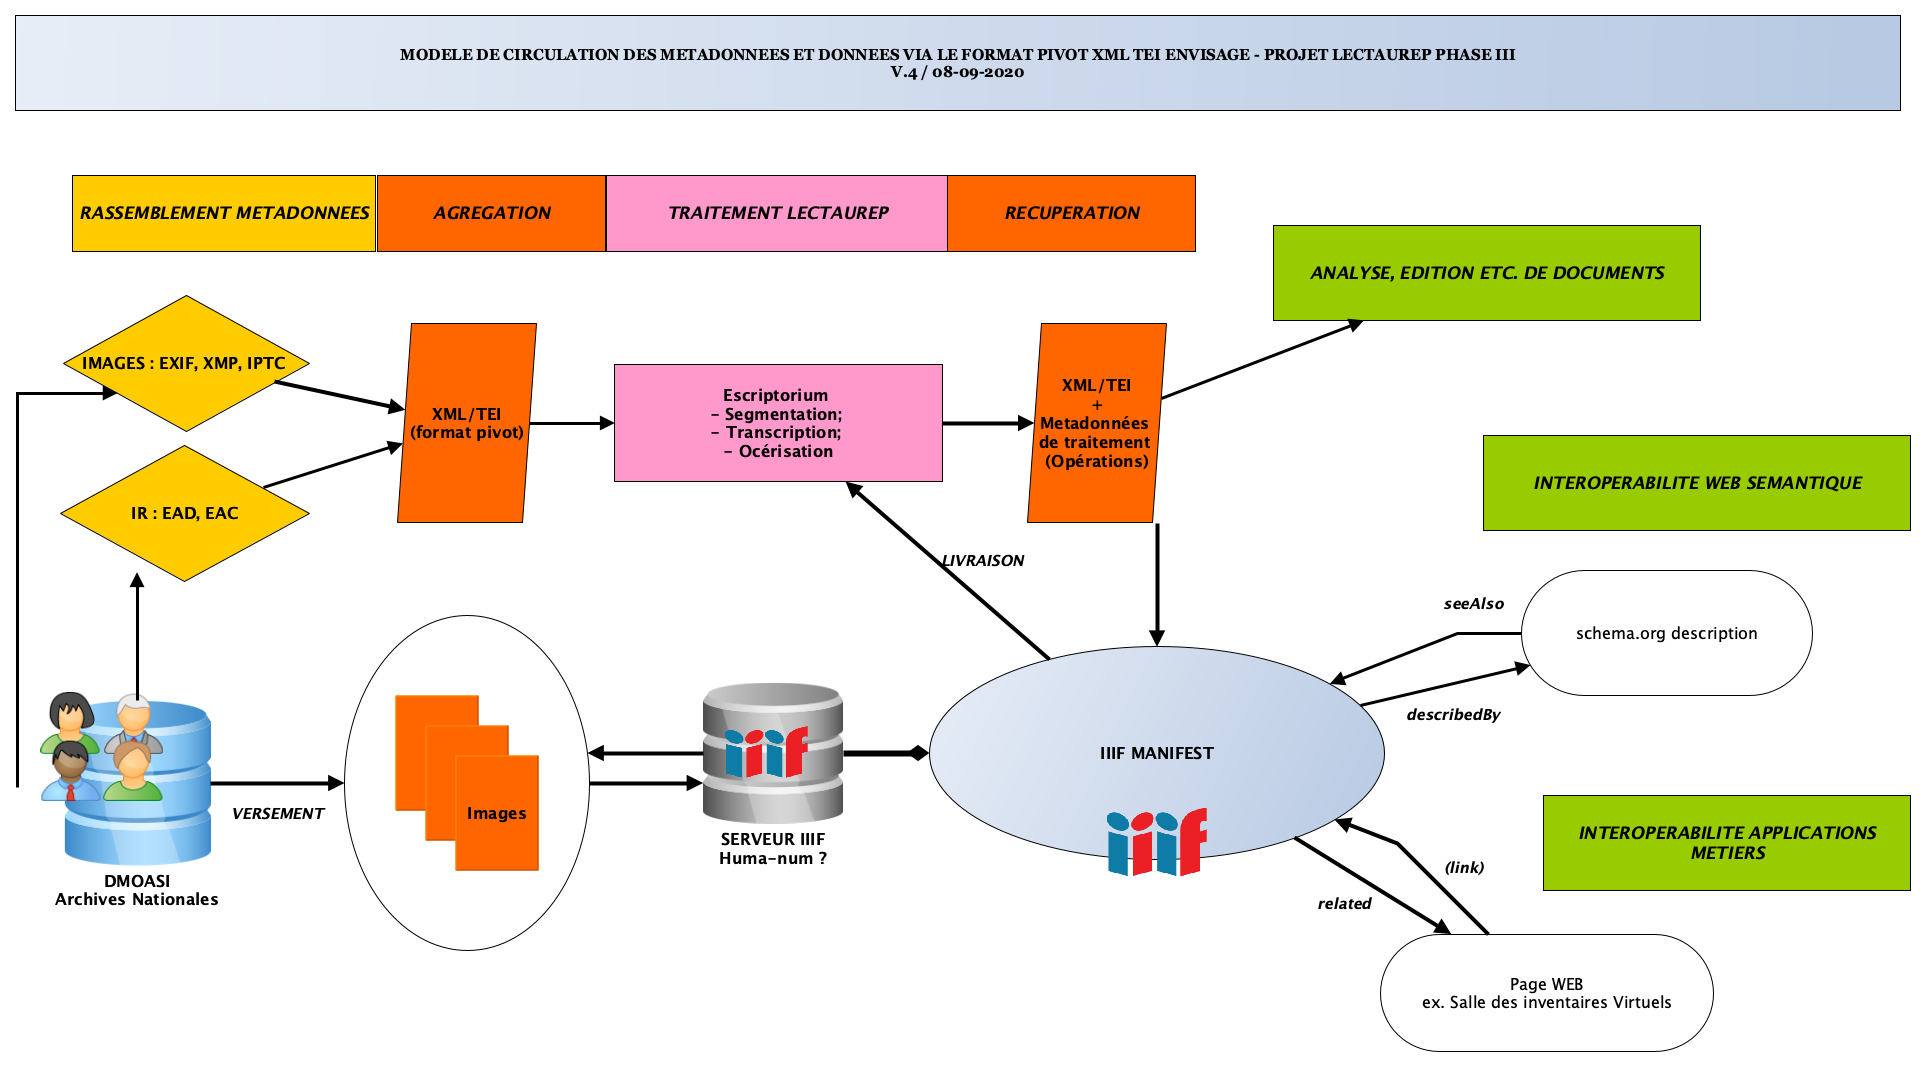
\includegraphics[width=18cm]{modèle_metadonnées_vise_V4}}}
    \caption{Schématisation du modèle de circulation des données dans eScriptorium souhaité par Lectaurep à terme  \textcopyright L. Terriel, 2020, yEd}
    \label{fig:modèle_métadonnées_vise_V4}
\end{figure}
\bigskip
Le format pivot XML est la solution qui a été envisagé pour permettre une intéropérabilité des formats, déjà en XML pour la plupart, et des spécifications des données Lectaurep dans eScriptorium. Il représente un bon point de départ pour traiter et agréger des flux entrants et sortants de données et de métadonnées hétérogènes dans une application client. Cependant, pour être opérationnel et intégrable, le format pivot doit répondre aux critères\footnote{Ces critères d'évaluation du format pivot sont adaptés de l'article \cite{stephane_standardisation_2006}} de : 
\begin{itemize}
    \item \inquote{délimitation} : simple à utiliser pour n'importe quel type d'applications, les données et métadonnées utilisées doivent être identifiables dans ce format;
    \item \inquote{soutenance} : intégrer à un environnement technique permettant son évolution (modification), son implémentation facile et sa documentation;
    \item \inquote{spécification} : chaque projet répond à des caractéristiques originales qui lui sont propres, cependant l'appui sur un schéma déjà existant et ouvert (modulable) permet de créer une ligne directrice, pour un développement rapide.
\end{itemize}
Nous verrons que si le format pivot peut sembler indéniable pour faire communiquer des données de différents SI dans Lectaurep, le choix de la spécification de ce format pivot s'avère en revanche moins évidente à définir (voir partie 3.2.2 et 3.2.3). 

\subsection{\inquote{Circonscrire un monde} de données}\label{Circonscrire un monde de données}

% mettre dans les annexes les documents : IR EAD et EAC, ALTO, 
% remonter schéma 
Avant de concevoir la mise en place d'un format pivot, il faut \inquote{circonscrire le monde}\footnote{\cite{poupeau_visite_2019}} des données et des métadonnées pour un projet. Cela implique dans un premier temps d'analyser les données et métadonnées, de comprendre leurs fonctionnements, leurs liens, d'établir la logique de ces liens et de les décrire. Pour établir les données que l'on aimerai retrouver lors d'un traitement dans eScriptorium. 
Le premier travail a consisté à repérer les données et les métadonnées qui pouvaient être, de prime abord en lien avec le minutier central et les archivistes, mais également de penser aux applications et usages futures de ces données et métadonnées. Une première approche consiste à modéliser les entrées et sorties des données et des métadonnées sous la forme d'un schéma qu'implique la transcription automatique par la plate-forme eScriptorium. 
\begin{figure}[h]
    \centering
    \centerline{\fbox{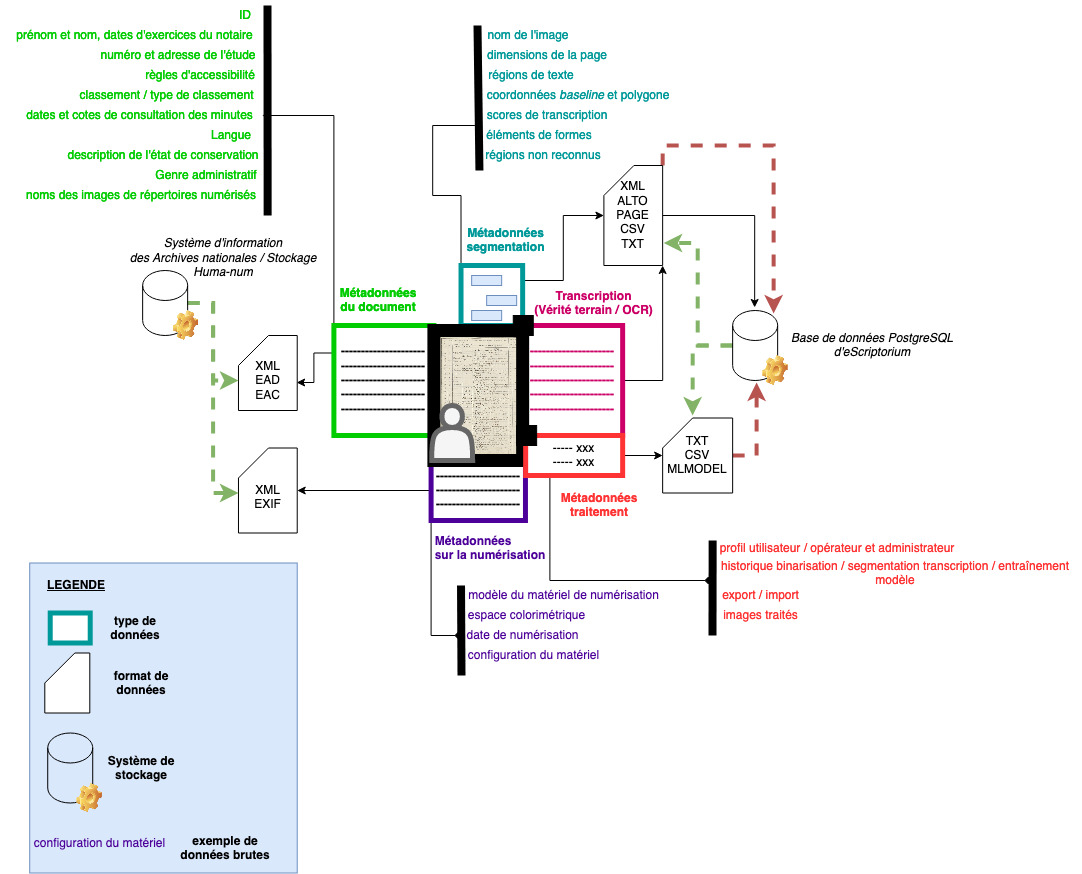
\includegraphics[width=15cm]{modélisation_données_lectaurep}}}
    \caption{Modélisation conceptuel des données, des formats et des systèmes d'informations du projet Lectaurep \textcopyright L. Terriel, 2020, drawio}
    \label{fig:modélisation_données_lectaurep}
\end{figure}

Nous distinguons donc des métadonnées inertes accompagnant la numérisation (peu succeptible de changer) : IR EAD, EAC, métadonnées numérisations

et les métadonnées changeantes et sortantes succeptibles d'évoluer dans le temps lors d'un traitement dans la plate-forme :
ALTO GT+coordonnées segmentation, compte utilisateurs, historiques des opérations, modèles d'entrainements produits avec le cli Kraken

nous l'avions déjà souligné plus haut point commun => encodage XML 
format TEI => large et modulable, acceuillir des évolutions

\section{Le format pivot XML TEI, un choix réaliste ?}

\subsection{La TEI (\inquote{Text Encoding Initiative}) pour annoter des données issu de l'éco-système Lectaurep}

La \textit{Text Encoding Initiative} (TEI) est sans doute l'un des projets d'application de l'informatique aux sciences humaines le plus important. Dans \inquote{40 ans de relations entre les sciences humaines et informatique}\footnote{Lou Burnard, \inquote{Du \textit{literary and linguistic computing} aux \textit{digital humanities} : retour sur 40 ans de relations entre sciences humaines et informatiques}, in \cite{mounier_dir_readwrite_2012}}, Lou Burnard, chercheur de l'Université d'Oxford, cofondateur de la TEI, fait remonter l'apparition du projet TEI au deuxième âge des humanités numériques situé au début des années 1980.  Après une période qu'il intitule \inquote{Litterary and linguistic Computing} marqué par les techniques statistiques de l'histoire quantitative, la TEI émerge dans la période des \inquote{Humanities Computing} : le chercheur s'éloigne alors du paradigme quantitatif (sans réellement le quitter\footnote{En 1983, la revue \textit{Histoire \& Mesure} parrait en France.}), pour maîtriser et développer le programme informatique lui-même et permettre son implémentation via la pratique du code. 
La TEI\footnote{Pour de plus de détails sur l'histoire, le fonctionnement et les usages de la TEI consulter \cite{burnard_quest-ce_2015}}, créée en 1987, vise à standardiser les pratiques d'encodage et de structuration des textes numérisés. Usité dans un premier temps dans le cadre du langage SGML, la TEI deviendra ensuite une norme d'encodage pour le langage XML applicable, en principe, à n'importe quelle source textuelle numérisée. L'outil est structuré par une communauté multidisciplinaire : historiens, linguistes, philologues, ou archéologues utilisent et adaptent cette norme selon leurs besoins en suivant les recommandations de l'un des 21 modules (550 éléments en 2015) des \textit{guidelines TEI P5}\footnote{Les \textit{guidelines TEI P5}, manuels, tutoriels, outils pour l'encodage de texte sont accessibles à l'adresse : \url{https://tei-c.org/guidelines/P5/}}. 
Il s'agit d'une avancée considérable évitant la sédimentation ou la \inquote{babélisation} numérique où chacun proposerai son propre langage d'encodage suivant sa propre théorie. Ce \inquote{métalangage} commun offre un cadre de travail et de structuration souple pour chaque projet ou discipline qui y retrouvent ses spécificités. Ce dispositif commun permet en particulier une intéropérabilité minimale entre les données, objectif apprécié et recherché dans le projet Lectaurep : au travers de la norme TEI, Lectaurep pourra encoder les informations des différents SI de l'éco-système Lectaurep (présenté plus haut dans 3.1.2) dans un format qui permet leur structuration, leur alignement (via des liens entre-elles), leur diffusion (vers d'autres formats de données ou d'autres programmes, par exemple) et leur archivage à long-terme. 


\subsection{Faire converger les standards de données vers un format pivot TEI, c'est confronter des visions opposées sur le document...}

Lors du colloque organisé aux Archives diplomatiques de La Courneuve, Seth Van Hooland rappelé en substance : \inquote{les standards de métadonnées et les ontologies sont comme les sous-vêtements, tout le monde est d'accord sur le fait qu'ils sont nécéssaires, mais personne ne veut utiliser le standard de quelqu'un d'autre.}\footnote{\cite{hooland_lapplication_2019} on trouve également une autre version de cette annecdote dans \cite{gillet_introduction_2016}, pp.102.}. Derrière l'affirmation humoristique et anecdotique du chercheur, repose une réalité pour les institutions patrimoniales : un musée, une bibliothèque, un centre d'archives et un chercheur porte un regard très différents sur les documents. Les spécifications sont ratachés à des usages métiers ancrés dans le temps.  Dans le projet ne pas minimiser la vision des acteurs de Lectaurep, dialogue entre les chercheurs, ingénieurs et archivistes est ici essentiel dans la mise en place d'un xml pivot
- philosophie différentes
- TEI module lourd pas forcément dans la logique de la description archivistique;
- nous l'avons vu EAD; EAC = TEI ? 
contrairement a EAD et EAC, TEI plus libre 


\subsection{...qui a pourtant fait ses preuves dans d'autres projets de standardisation et présente des qui présente des avantages pour Lectaurep}

faire comprendre qu'on utilise pas ce format pour de l'édition mais comme format passerèlle entre
Nous avons vu plus haut que des projets d'éditorialisation aux AN rendé la TEI tout à fait compatible avec la description archivistique, mais au-delà de donner à voir le texte, la TEI présente les avantages de pouvoir ...
comme 
plate-forme de publications scientifiques :

- Istex
- Hal 
- Office national des brevets

La TEI peut faire office de dénominateur commun 

Les avantages d'un format de données unifiées pour l'alignement des données

Ouvrir les répertoires de notaires à d'autres visualisations
- permettre IIIF
-> manipuler données vers d'autres applications (TAL, Edition...)
Projets des AN :

- Himanis
- Testaments de poilus
- edition des répertoires de notaires
- créer un espace pour un référentiel de mains
- annotation faciliter avec TEI
- permettre des études paléographiques dans la lignée des sites (Marc Smith). La TEI permet l'encodage des mains avec l'élément Hand Desc

Anticiper les cas d'usages du métier d'archiviste




- pérénisation passe par une veille sur l'évolution des standards 
- harmoniser et moderniser les IR : pouvoir rattacher les données issues de lectaurep aux IR
- rétroconversion (Lupovici catherine) vers des standards archivistiques plus récent EAD 3 et RIC-O ? 

=> problèmatiques + objectifs = TEI tout indiqué 

Le chapitre suivant décrit le workflow de travail mis en place pour le format pivot TEI, la figure \ref{fig:workflow_tei_pivot_lectaurep} résume ces différentes étapes.

\begin{figure}[h]
    \centering
    \centerline{\fbox{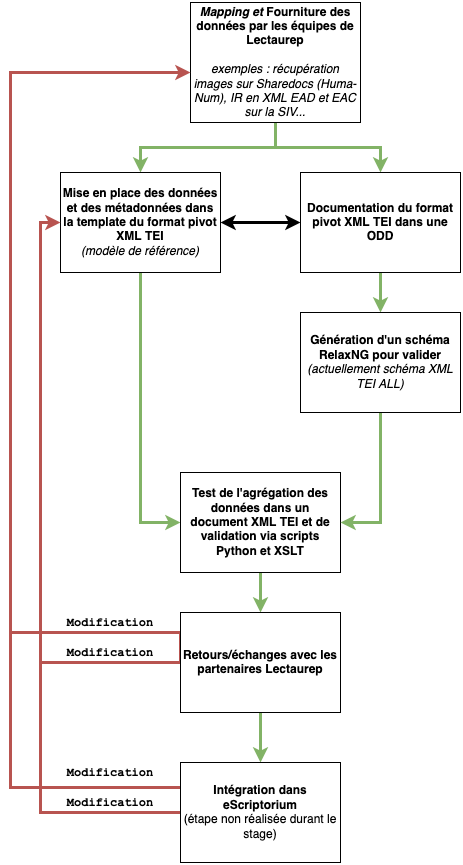
\includegraphics[width=8cm]{workflow_tei_pivot_lectaurep}}}
    \caption{Présentation du workflow pour le format pivot XML TEI Lectaurep mis en place durant le stage  \textcopyright L. Terriel, 2020, drawio}
    \label{fig:workflow_tei_pivot_lectaurep}
\end{figure}

\chapter{Présentation du \textit{workflow} et mise en place d'une première version du format pivot XML-TEI de Lectaurep}

\section{Une \textit{template} XML TEI, un fichier XML dans un environnement partagé et ouvert}
% accroche
Une fois la modélisation des données élaborée et les objectifs du format pivot XML TEI formalisés; il est nécessaire de concevoir le format pivot XML TEI lui-même. 
% objectifs
Pour synthétiser et visualiser l'exposition des multiples données Lectaurep dans des champs TEI; il fallait disposer d'un fichier de travail XML suffisamment modulable et ouvert.
Ceci pour synthétiser et inclure les nouvelles réflexions des acteurs qui ont cours au gré des discussions et des réunions autour de la récupération de tel ou tel données, mais également pour permettre l'insertion ou la suppression de tel ou tel nouvel élément TEI appartenant aux \textit{guidelines TEI P5}.
On parle alors de mode de développement pour la conception du pivot XML TEI : par le biai d'une \textit{template} XML TEI, entendu ici comme un canevas ou encore un fichier de travail prêt à l'emploi, on autorise un grand nombre de modifications à l'intérieur de ce fichier jusqu'à atteindre son état logique, stable et finalisé. 
% Création de la template
Pour créer la \textit{template} XML TEI, nous sommes parti d'un fichier XML TEI (All) (Cf. Figure \ref{fig:document_minimal_tei}) généré à partir de l'éditeur XML Oxygen. Il s'agit d'un \textit{framework}, présentant une structure minimal en TEI comprenant l'élément racine \citecode{<TEI>} et les deux sous-éléments \citecode{<teiHeader>} et \citecode{<text>}, valide du point de vue d'un schéma Relax NG (REgular LAnguage for XML Next Generation) englobant l'intégralité de la TEI.
La possibilité de revenir régulièrement sur la structure de cette \textit{template} TEI et de créer, à terme, son propre schéma, grâce à ce \textit{framework} constituent des avantages pour Lectaurep dans la suite du projet.    
\begin{figure}[h]
    \centering
    \centerline{\fbox{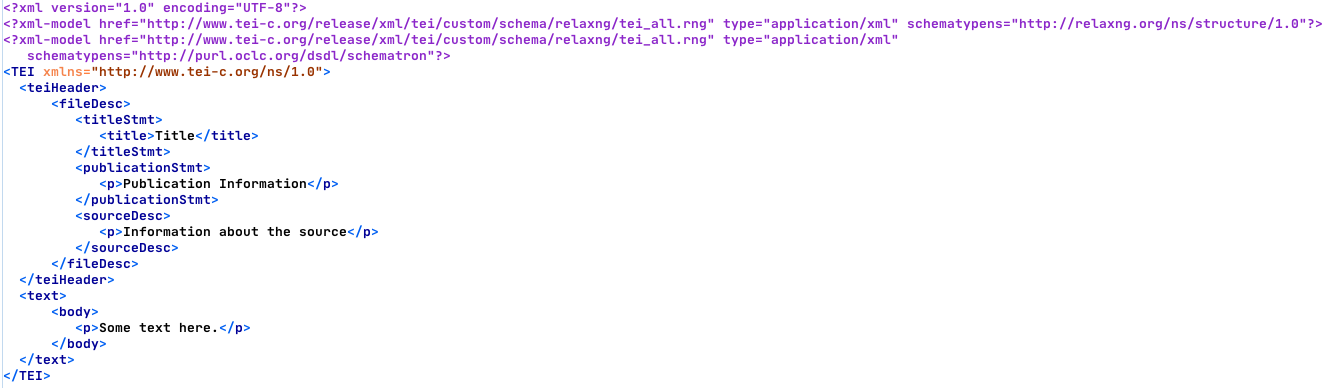
\includegraphics[width=19cm]{document_minimal_tei}}}
    \caption{Document XML TEI minimal conforme et valide  \textcopyright L. Terriel, 2020, Oxygen XML Editor}
    \label{fig:document_minimal_tei}
\end{figure}


\newpage
% Environnement de partage de la template
Pour mettre en relation et coordonner les acteurs du projet autour de la \textit{template} TEI et prévoir des retours de leurs part, il a été décidé de placer ce fichier dans la plate-forme GitLab \footnote{la \textit{template} du format pivot TEI pour Lectaurep est consultable en ligne dans son entier via : \url{https://gitlab.inria.fr/almanach/lectaurep/documentation/-/blob/master/Doc/Modélisation_et_schémas_de_validation/template_pivot_TEI_lectaurep.xml} [une permission peut-être demandée] sinon Cf. Annexe} dans le dépôt rassemblant la documentation et les tests effectués à partir de ce format pivot XML TEI. Cet environnement permet d'avoir des suggestions d'améliorations sous la forme de billets (\textit{issues}) et d'assurer une traçabilité des évolutions et des versions du format pivot, par le biais des \textit{commits}, qui permettent de constitué un historique des soumissions et des modifications effectuées sur ce fichier au fur et à mesure de l'avancement. 
\newpage

\section{Une première version du schéma pour le format pivot XML TEI qui s'appuie sur un repérage et des choix d'imbrications (\textit{mapping}) et sur la conversion de champs équivalents (\textit{crosswalk schema})}

% Règles préalables 

Afin de proposer une première structuration de la \textit{template} du format pivot XML TEI, nous avons décidé, en coordination avec le DMC, de nous concentrer en premier lieu sur le \textit{mapping}\footnote{Nous entendons ici le \textit{data mapping} comme le procédé qui consiste à extraire des données provenant de standards différents qui seront exposées dans le format pivot XML TEI pour permettre leurs récupération dans d'autres systèmes d'informations.} et la fourniture des données appartenant aux catégories suivantes (pour le détail des données et des éléments retenus selon les spécifications Cf. Table \ref{table:mapping_données_lectaurep}) :  

\begin{itemize}
    \item \textbf{Métadonnées de gestion et de description essentielles} : correspondant aux données extraites des instruments de recherche en XML EAD et EAC fournis par le DMC et disponibles sur la SIV;
    \item \textbf{Métadonnées techniques des images} : correspondant aux données contenus dans les images, répondant à la spécification EXIF et extraites via un outil d'édition image ou un script Python;
    \item \textbf{Images} : essentiellement les noms des fichiers images stockés sur un serveur Humanum (ShareDocs);
    \item \textbf{Données provenant des traitements HTR} : correspond aux transcription de vérité terrain, exportés depuis sur la plate-forme eScriptorium, au format XML ALTO;
\end{itemize}

A première vue ce choix peut paraître arbitraire, dès lors pourquoi ne pas avoir pris en compte les données correspondant aux modèles de segmentation utilisés sur eScriptorium pour les documents de vérités terrains ? Où sont les transcriptions issues de la reconnaisance automatique ? pourquoi ne pas avoir pris en compte les éléments diplomatiques ? voici deux éléments de réponses simples : soit les  données n'existaient pas encore, comme dans le cas des transcriptions HTR ou des éléments diplomatiques, de plus la durée du stage ne permettait pas la prise en compte de la récupération complexe des métadonnées correspondant aux modèles de segmentation HTR au moment de l'élaboration du format pivot. 

La première mise à plat des données proposée plus haut présente les avantages suivants dans la réalisation du format pivot : 
\begin{itemize}
    \item Facilité d'accès aux données;
    \item Set de données de taille moyenne, évitant la dispersion dans la représentation TEI et la redondance de données, dans cette première expérimentation;
    \item Proposer une première hiérarchisation (Cf. Figure \ref{fig:oignon_diagram_niveaux_donnees_lectaurep}) des données dans le futur encodage XML TEI, avec quatre niveaux bien distincts, allant du plus au degré de granularité (métadonnées liées aux images et aux répertoires de notaires physiques) au plus bas degré qui est le texte de vérité terrain.
\end{itemize}

\bigskip

\begin{center}
\begin{figure}[h]
    \centering
    \centerline{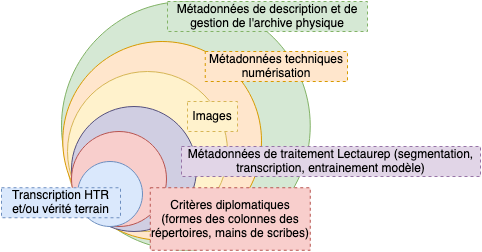
\includegraphics[width=13cm]{oignon_diagram_niveaux_donnees_lectaurep}}
    \caption{Diagramme en oignon des différents niveaux de granularité des données Lectaurep pour représenter les imbrications dans le format pivot XML TEI \textcopyright L. Terriel, 2020, drawio}
    \label{fig:oignon_diagram_niveaux_donnees_lectaurep}
\end{figure}
\end{center}

\newpage
%---------------------------------
%% TABLEAU : Mapping des principales données Lectaurep utilisées pour la première version du format pivot XML TEI
\begin{center}
\begin{longtable}{|p{3cm}|p{2.5cm}|p{5cm}|p{5.5cm}|}
% légende et label du tableau
\caption{\textit{Mapping} des principales données Lectaurep utilisées pour la première version du format pivot XML TEI} 
\label{table:mapping_données_lectaurep}

% ligne de titres du tableau
\hline
\rowcolor[RGB]{220, 220, 220} % gris
\textbf{CATÉGORIES} & \textbf{SCHÉMAS} & \textbf{DONNÉES} & \textbf{ELEMENTS XML} \endhead
        
% gestion du footer        
\hline \rowcolor[RGB]{220, 220, 220} \multicolumn{4}{|r|}{{Continue sur la page suivante \hookrightarrow}} \\ \hline
\endfoot
\hline \hline
\endlastfoot
        
        % Métadonnées EAD
        \hline
        \rowcolor[RGB]{88, 214, 141} % vert
        \footnotesize{\textbf{Métadonnées de gestion et de description}} & \footnotesize{EAD} & \footnotesize{Noms des fichiers EAD} & \footnotesize{\citecode{<eadid>}} \\
        \cline{3-4}
        \rowcolor[RGB]{88, 214, 141}
        & & \footnotesize{Nom et prénom du notaire} & \footnotesize{\citecode{<persname>}} \\
        \cline{3-4}
        \rowcolor[RGB]{88, 214, 141}
        & & \footnotesize{Étude du notaire} & \footnotesize{\citecode{<corpname>}} \\
        \cline{3-4}
        \rowcolor[RGB]{88, 214, 141}
        & & \footnotesize{Composant pour la description du niveau répertoire} & \footnotesize{\citecode{<c level="series">}} \\
        \cline{3-4}
        \rowcolor[RGB]{88, 214, 141}
        & & \footnotesize{Sous-composant pour la description du niveau minutes} & \footnotesize{\citecode{<c level="recordgrp">}} \\
        \cline{3-4}
        \rowcolor[RGB]{88, 214, 141}
        & & \footnotesize{Cotes des composants et des sous-composants de description} & \footnotesize{\citecode{<unitid type="cote-de-consultation">}} \\
        \cline{3-4}
        \rowcolor[RGB]{88, 214, 141}
        & & \footnotesize{Intitulé des composants et des sous-composants de description} & \footnotesize{\citecode{<unittitle>}} \\
        \cline{3-4}
        \rowcolor[RGB]{88, 214, 141}
        & & \footnotesize{Dates des composants et des sous-composants de description} & \footnotesize{\citecode{<unitdate>}} \\
        \cline{3-4}
        \rowcolor[RGB]{88, 214, 141}
        & & \footnotesize{Description physique des documents compris dans les composants et des sous-composants de description} & \footnotesize{\citecode{<physdesc>}} \\
        \cline{3-4}
        \rowcolor[RGB]{88, 214, 141}
        & & \footnotesize{Informations supplémentaires sur les composants et des sous-composants de description} & \footnotesize{\citecode{<scopecontent>}} \\
        
        % Métadonnées EAC
        \cline{2-4}\rowcolor[RGB]{88, 214, 141}
        & \footnotesize{EAC} & \footnotesize{Dates d'exercices du notaire} & \footnotesize{\citecode{<dateRange>} > \citecode{<fromDate>} / \citecode{<toDate>}}\\
        
        % Métadonnées EXIF
        \hline\rowcolor[RGB]{230, 126, 34} % orange
        \footnotesize{\textbf{Métadonnées techniques des images numérisées}} & \footnotesize{EXIF} & \footnotesize{Titre de la numérisation} & \footnotesize{\citecode{<EXIF:ImageDescription>}} \\
        \cline{3-4}
        \rowcolor[RGB]{230, 126, 34}
        & &  \footnotesize{Version du standard Exif} & \footnotesize{\citecode{<EXIF:ExifVersion>}} \\
        \cline{3-4}
        \rowcolor[RGB]{230, 126, 34}
        & &  \footnotesize{Nom du constructeur de l'équipement} & \footnotesize{\citecode{<EXIF:Make>}} \\
        \cline{3-4}
        \rowcolor[RGB]{230, 126, 34}
        & &  \footnotesize{Nom du modèle de l'équipement} & \footnotesize{\citecode{<EXIF:Model>}} \\
        \cline{3-4}
        \rowcolor[RGB]{230, 126, 34}
        & &  \footnotesize{Orientation de l'image en terme de colonnes et lignes} & \footnotesize{\citecode{<EXIF:Orientation>}} \\
        \cline{3-4}
        \rowcolor[RGB]{230, 126, 34}
        & &  \footnotesize{Nombre de pixels par résolution (\citecode{<EXIF:ResolutionUnit>}) en fonction de la largeur} & \footnotesize{\citecode{<EXIF:XResolution>}} \\
        \cline{3-4}
        \rowcolor[RGB]{230, 126, 34}
        & &  \footnotesize{Nombre de pixels par résolution (\citecode{<EXIF:ResolutionUnit>}) en fonction de la longueur} & \footnotesize{\citecode{<EXIF:YResolution>}} \\
        \cline{3-4}
        \rowcolor[RGB]{230, 126, 34}
        & &  \footnotesize{Unité de mesure de \citecode{<EXIF:XResolution>} et \citecode{<EXIF:YResolution>}} & \footnotesize{\citecode{<EXIF:ResolutionUnit>}} \\
        \cline{3-4}
        \rowcolor[RGB]{230, 126, 34}
        & &  \footnotesize{Date de dernière modification} & \footnotesize{\citecode{<EXIF:ModifyDate>}} \\
        \cline{3-4}
        \rowcolor[RGB]{230, 126, 34}
        & &  \footnotesize{Position des composantes de chrominance par rapport à la composante de luminance. S'applique uniquement aux données compressées de type JPEG. La valeur par défaut est 1} & \footnotesize{\citecode{<EXIF:YCbCrPositioning>}} \\
        \cline{3-4}
        \rowcolor[RGB]{230, 126, 34}
        & &  \footnotesize{Date et heure du stockage de l'image comme donnée numérique} & \footnotesize{\citecode{<EXIF:DateTimeDigitized>}} \\
        \cline{3-4}
        \rowcolor[RGB]{230, 126, 34}
        & &  \footnotesize{Date et heure du stockage de la création de l'image} & \footnotesize{\citecode{<EXIF:DateTime>}} \\
        \cline{3-4}
        \rowcolor[RGB]{230, 126, 34}
        & &  \footnotesize{Informations spécifiques aux données compressées} & \footnotesize{\citecode{<EXIF:ComponentsConfiguration>}} \\
        \cline{3-4}
        \rowcolor[RGB]{230, 126, 34}
        & &  \footnotesize{Si EXIF supporte Flashpix format Ver. 1.0, une valeur par défaut '0100' est inscrite sinon 'NULL'} & \footnotesize{\citecode{<EXIF:FlashpixVersion>}} \\
        \cline{3-4}
        \rowcolor[RGB]{230, 126, 34}
        & &  \footnotesize{Spécifications sur l'espace colorimétrique de l'image} & \footnotesize{\citecode{<EXIF:ColorSpace>}} \\
        
        % Métadonnées ALTO
        \hline\rowcolor[RGB]{52, 152, 219} % bleu
        \footnotesize{\textbf{Données correspondant au document vérité terrain}} & \footnotesize{ALTO} & \footnotesize{Représentation de l'image} & \footnotesize{\citecode{<Layout>}}  \\
        \cline{3-4}
        \rowcolor[RGB]{52, 152, 219}
        & &  \footnotesize{Une page de répertoire} & \footnotesize{\citecode{<Page>}} \\
        \cline{3-4}
        \rowcolor[RGB]{52, 152, 219}
        & &  \footnotesize{Rectangle couvrant la zone imprimée d'une page} & \footnotesize{\citecode{<PrintSpace>}; les coordonnées spatiales de l'élément et les dimensions est donné par les attributs \citecode{@HPOS, @VPOS, @WIDTH, @HEIGHT}} \\
        \cline{3-4}
        \rowcolor[RGB]{52, 152, 219}
        & &  \footnotesize{Bloc de texte qui regroupe les lignes de textes} & \footnotesize{\citecode{<TextBlock>}} \\
        \cline{3-4}
        \rowcolor[RGB]{52, 152, 219}
        & &  \footnotesize{Ligne de texte} & \footnotesize{\citecode{<TextLine>}, elle contient la \textit{baseline} du texte sous la forme de points via l'attribut \citecode{@BASELINE}; les coordonnées spatiales de l'élément et les dimensions est donné par les attributs \citecode{@HPOS, @VPOS, @WIDTH, @HEIGHT}} \\
        \cline{3-4}
        \rowcolor[RGB]{52, 152, 219}
        & &  \footnotesize{Forme de délimitation d'une ligne de texte, si elle n'est pas rectangulaire} & \footnotesize{\citecode{<Shape>}} \\
        \cline{3-4}
        \rowcolor[RGB]{52, 152, 219}
        & &  \footnotesize{Contenu par \citecode{<Shape>}, décrit une forme polygonale} & \footnotesize{\citecode{<Polygon>}, les points sont décrits par l'attribut \citecode{@POINTS}} \\
        \cline{3-4}
        \rowcolor[RGB]{52, 152, 219}
        & &  \footnotesize{Chaîne de caractères de la ligne de texte et leurs positions} & \footnotesize{\citecode{<String>}, les chaînes de caractères de caractères sont comprises dans l'attribut \citecode{@CONTENT}; les coordonnées spatiales de l'élément et les dimensions est donné par les attributs \citecode{@HPOS, @VPOS, @WIDTH, @HEIGHT} identique à \citecode{<TextLine>}} \\
        
\end{longtable}
\end{center}
%---------------------------------
\newpage

% Organisation détaillé et difficultés

L'étape suivant le repérage et l'imbrication des données consistait à répondre à la question suivante : à quel élément TEI faire correspondre tel ou tel élément de Lectaurep ? Une solution consisté à commencer par le haut de l'arbre TEI puis à descendre petit à petit dans l'arbre en prenant les éléments les uns après les autres. Cependant les éléments de Lectaurep appartenant à trois niveaux de granularités différents, nous devions disposer d'une architecture plus concrète (que le \textit{framework} TEI ALL) pour disposer ensuite les éléments uns à uns dans le format pivot (Cf. Figure \ref{fig:structure_general_template_tei_lectaurep}) : la balise \citecode{<teiHeader>}\footnote{\cite{tei_tei_nodate}} pour encoder la partie la plus théorique, correspondant aux métadonnées relatives aux archives physiques et aux images (données issues des fichiers XML EAD/EAC et EXIF), la balise \citecode{<facsimile>}\footnote{\cite{tei_tei_nodate-2}} pour recevoir les coordonnées (données issues des fichiers XML ALTO) et faire le pont entre les métadonnées générales du \citecode{<teiHeader>} et le \citecode{<text>} par un système d'identifiants, et la balise \citecode{<text>}\footnote{\cite{tei_tei_nodate-1}} pour accueillir le texte issu du document de vérité terrain (données égallement issues des fichiers XML ALTO). 

\begin{figure}[h]
    \centering
    \centerline{\fbox{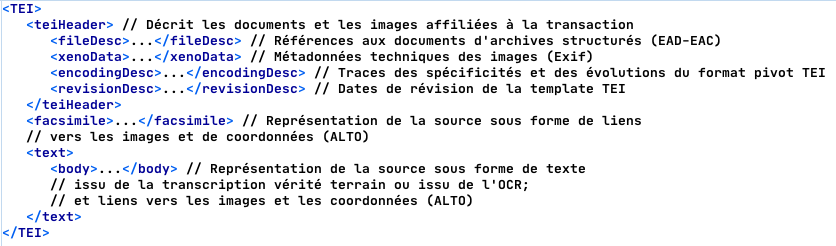
\includegraphics[width=19cm]{structure_general_template_tei_lectaurep}}}
    \caption{Schéma minimal retenu pour l'exposition des données Lectaurep dans un format pivot XML TEI \textcopyright L. Terriel, 2020, Oxygen XML Editor}
    \label{fig:structure_general_template_tei_lectaurep}
\end{figure}

% 1. teiHeader : conversion EAD - EAC vers TEI

La conversion EAD n'a pas présenté de réel difficulté, en effet certains éléments EAD se retrouve explicement dans la TEI et de plus crosswalks 
valeurs par défaut 

% 2. teiHeader : Exif vers TEI via Xenodata

% 3. pour permettre le suivi des modifications et choix d'encodage : <encodingDesc> et <revisionDesc>

% 4. facsimile / text : ALTO

Voir la note pour l'élement TEI <path> qui doit être rejeté pour <zone> si polygone

\begin{figure}[h]
    \centering
    \centerline{\fbox{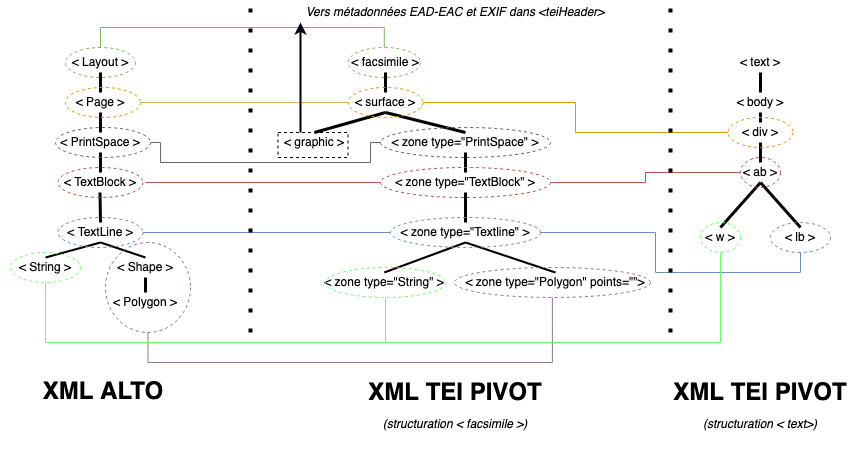
\includegraphics[width=19cm]{Structuration_arbre_alto_tei_liens.png}}}
    \caption{Structure du fichier XML ALTO à gauche et du fichier XML TEI pivot et liens entre les éléments \textcopyright L. Terriel, 2020, drawio}
    \label{fig:structure_arbre_tei_alto}
\end{figure}



  
% liaison entre les parties
Les objectifs étaient les suivant créé un fichier xml intégrant une architecture TEI suffisament générique et large de manière à pouvoir inbsérer par la suite de nouveaux types de données et spécifier des contraintes. Cela pourrai ressembler un entenoir. 
récupération des id
Afin d'éviter la redondance de données nous avons décidé et de remplir abondament la template, Difficulté pour les EAD /EAC pour les EAC contenant finalement des informations redondantes avec les EAD, nous avons choisi seulement de reporter l'ID de tel manière, entrée vers liens RDF (représenté ) et les voacbulaires (term vocabularySource)





les liens entre ces deux parties s'effectue via des id de la manière suivantes

- le but fixé lors du stage et grâce aux différents retour des réunions => 
- mise en place du dépot et des feedbacks sous forme d'issue = dans le cadre d'une approche agile
- très ouvert TEI ALL 

template => faire tableau équivalents éléments + arbre
choix des données à utilisés - crosswalks - littérature

grosse limites !!! 
a améliorer voir ODD 

\section{Une ODD pour documenter, partager et valider la \textit{template} XML TEI}

% résumer les évolutions 

- Distinguer via un atteribut les Alto transcriptions OCR et vérité terrain 
- proposer 
- tests de récupération sur eScriptorium en TEI des images et de leurs métadonnées 


Partager le XML au sein d'une communauté ODD
dans la pratique il n'est pas conseillé d'utiliser un schéma TEI ALL, cependant il reste encore beaucoup d'éléments à intégrer ... éléments diplomatiques handdesc (mains) reliés à ces cotes et au support de numérisation 
entonir
La méthodologie que nous avons mis en place est la création d'une \textit{template} (ou canevas) XML TEI afin de créer une architecture suffisamment générique pour permettre l'inclusion a posteriori de contraintes sous la forme d'un entonoir qui doit aboutir à la mise en place d'un schéma validant et restreint. 

\section{Simuler l'agrégation des données et la validation d'un fichier XML TEI}
- ne parle forcément aux archivistes;
- besoin de visualiser les données dans un canevas TEI et d'envisager;
- besoin de valider en cas de changement dans l'ODD; 

= > CLI Python pour générer un format pivot XML TEI et valider grâce à un schéma RELAX NG
1- CVS
2- Données de tests + schéma TEI ALL
3- Algorigrammes 
4 - XSLT (fonctionnement et crosswalks disponibles) et fonction collection article - difficulté oxygen usage de la fonction os.popen avec Saxon 
